\begin{figure}[htbp]
  \centering
  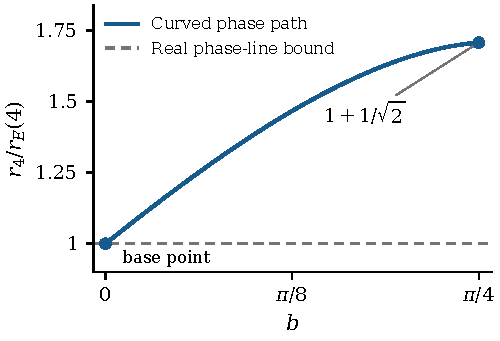
\includegraphics[width=\columnwidth]{figures/fig3_curved.pdf}
  \caption{$n=4$ 时沿显式弯曲相位路径的增强。
  实线由闭式根在 $0\leq b\leq\pi/4$ 上直接计算得到，满足
  $r_4/r_E(4)=\cos[b+\delta(b)]-\sin\delta(b)$，从 $1$ 严格增至 $1+1/\sqrt2$。
  水平虚线表示所有经过指定基点的实相位直线的半径上界。 绘图代码由 OpenAI Codex（GPT-6）辅助编写，并按文中公式核对。}
  \label{fig:curved}
\end{figure}
